\chapter{Purpose}
\label{chap:purpose}

As was mentioned in Chapter \ref{chap:intro}, Custos aims to provide
dedicated secret storage and access control system. In doing so, it
hopes to solve the cryptographic key storage problem, making
encryption easier to use and more widely available to the average
user. To accomplish this goal, Custos must be both usable and secure.
Furthermore, it must be flexible enough to support a range of modern
use cases. In this chapter, I'll discusses the goals Custos hopes to
achieve, a number of possible application where Custos can help secure
data, and the threat model that Custos assumes.

\section{Goals}

Custos's primary goal is as stated above: ``To provide secure, easily
usable, secret storage and access control''. This entails
accomplishing a number of sub-goals: providing secret storage, making
it easy to use, and ensuring security.

\subsection{Secret Storage}

Custos is a secret store. As such, it had better be cable of storing
secrets. Custos does this using standard object-storage key:value pair
semantics. I expect most Custos implementations (including the ones
described in this document) to defer the actual key:value storage
aspect of Custos to existing key:value storage systems. Why reinvent
the wheel? Instead, we must identify what key:value storage
capabilities are desirable in a Custos back end. The primary drivers
of this analysis are the type of data Custos will store, and the
methods in which this data will be accessed. We already know that
Custos will often be used to store key:value pairs mapping data
identifiers (the keys) to corresponding encryption keys (the
values). As far as accessing this data goes, I would expect access
patterns similar to that of the encrypted data that Custos is being
used to protect. Most modern data, including the personal data that
I'd expect users to use encryption and Custos to protect, follows an
append-only, read-heavy workload~\cite{Ghemawat2003}.

With these thoughts in mind, I propose the following as desirable
traits for a the key:value storage components of Custos.

\begin{packed_desc}
\item[Fast Access] \hfill \\ A user will likely not accept too much
  overhead having to wait on Custos when wishing to access their
  encrypted data. Thus, Custos should strive to provide quick access
  to key:value pairs. If a compromise must be made between read and
  write speed, read speed should be favored since reads will likely
  outnumber writes.
\item[Versioned Data] \hfill \\ When data is updated, it is likely
  that the user may wish to re-encrypt it with a new key (more on this
  in later sections). As such, Custos should support storing multiple
  versions of the value associated with a given key.
\item[Arbitrary Data] \hfill \\ Encryption keys and other secrets come
  in a variety of shapes, sizes, and formats. To support the maximum
  range of encryption systems, Custos should allow the storage of
  arbitrary binary data associated with a given UUID key.
\end{packed_desc}

\subsection{Usability}

As we discussed in Chapter \ref{chap:intro}, Custos aims to achieve
usability across three discreet usage types: the usability of
encryption systems leveraging Custos (end-user usability), the
usability of Custos to manipulate access control mechanisms
(administrative usability), and the ease with which Custos can be
interfaced with other systems (developer usability).

On the end user usability front, Custos aims to expand the
accessibility of encryption systems be providing flexibility. It aims
to provide a more natural match between desired uses for cryptography
and attainable uses of cryptography, narrowing the intention vs
capability divide. As such, Custos aims to enable encryption system to
support the following attributes of successful modern storage systems.

\begin{packed_desc}
\item[Multi-Device Support] \hfill \\ Today a given users tends to
  have multiple computing devises. And they expect to by able to sync
  their data across these devices and access it from each regardless
  of whether or not it is encrypted. Thus, Custos must support this
  form of multi-device access where the data may be decrypted and read
  from a device other than the one on which it was originally
  encrypted.
\item[Multi-User Support] \hfill \\ We like to share. User's today
  expect to be able to share files or data with their friends or
  coworkers and access data others have shared with them. Custos must
  support the ability to share encrypted files with other users,
  granting the necessary users access to the corresponding encryption
  keys so that they might decrypt and access the shared data.
\item[Flexible Protection Semantics] \hfill \\ Some data requires only
  cursory protections and should allow wide ranging access, other data
  requires moderate protection but should still allow access by a
  large group of Friends. Still other data should never be accessed by
  anyone other than its creator. Custos must support a range of
  security levels, allowing the user to select the appropriate point
  on the security vs accessibility continuum.
\end{packed_desc}

In addition to end-user usability, Custos also aims for administrative
usability, making it easy to control access to one's data. Custos aims
to achieve this goal by providing users with the ability to grant
access on the basis of a variety of authentication parameters,
creating a flexible and straightforward system for controlling access
to encryption keys, and by proxy, the data they protect. The following
characteristics will help ensure Custos remains usable from an
administrative perspective.

\begin{packed_desc}
\item[Flexible Authentication Mechanisms] \hfill \\ Some data need
  only be protected by a simple check of what IP address wishes to
  access it, other data requires an interactive password prompt to
  access, still other data access may require a password prompt and
  possession of a multi-factor device like a cell phone. Users should
  be able to select how their data is protected and what hurdles must
  be jumped to access it.
\item[Simple Access Control] \hfill \\ The semantics for granting a
  specific actor access to specific data for a specific capability
  should be simple and straightforward. It should be clear how to
  grant access, what level of security that access entails, and what
  the grantee is able to do with such access. Occasionally, you will
  need to revoke access that has been previously granted. Doing so
  should also be simple and have well defined semantics to ensure the
  user knows what effect revoking access is guaranteed or not
  guaranteed to have.
\item[Logical Centralization] \hfill \\ A Custos server should appear
  as a centralized, globally accessible resource. This will allow
  applications to access a Custos server regardless of their relative
  locations. There are some situations where administrators may wish
  forgo truly global access in favor of operating a Custos server in a
  manner that limits access to specific networks or resources, but
  even in these cases a Custos server should be treated as a global
  resource within any given administrative domain.
\end{packed_desc}

The final component of Custos usability is its developer usability. If
we are to expect Custos to be integrated into existing cryptographic
products, it must be easy for developers to accomplish this
feat. Custos aims to maintain a high degree of developer usability via
the following features.

\begin{packed_desc}
\item[Well Defined API] \hfill \\ Custos will expose a standard API
  for data access and administrative management. This API will provide
  a well defined interface for interacting with a Custos server,
  regardless of server provider or implementation.
\item[Standard Design Patterns] \hfill \\ The Custos API will attempt
  to adhere to standard web-based design patterns by implementing a
  REST-based architecture~\cite{ibm-restful}. This bring all of the
  standard usability benefits of RESTful systems (statelessness, etc)
  while also being a well understood architecture to develop against.
\item[Standard Data Formats] \hfill \\ Custos aims to support
  arbitrary data storage. But it will do so using commonly deployed
  data standards like JSON~\cite{json} and Base64 encoding. There are
  a variety of libraries available to deal with these formats, making
  it easy to convert between Custos API messages and native internal
  data types for client applications in a variety of languages.
\end{packed_desc}

\subsection{Security}

Being a secure secret store means that Custos must be... secure.  In
addition to the ``increased security through increased usability''
items discussed above, what does it mean to be a secure secret store?
Does it mean that the secrets are stored in a manner that ensures they
remain secure in the event of a server breach? Does it mean that the
server operator has no ability to access user secrets directly. Does
it merely mean the access to secrets is well controlled?

We discuss Custos's security model in detail later in this chapter,
but Custos adopts the last of the previous questions as the basis for
its definition of a secure secret store. A key value storage is
secure if access to secrets is well regulated. To achieve this
level regulation, Custos requires several traits:

\begin{packed_desc}
\item[Secure Communication Primitives] \hfill \\ The Custos API must
  be protected against eavesdropping and Man-In-The-Middle
  attacks. Custos leverages SSL and the existing PKI systems to
  achieve this.
\item[Access Control] \hfill \\ Custos provides the ability to
  regulate key access in a variety of flexible means (see above). It
  provides access control at a variety of levels, and provides support
  for versioning and revocation.
\item[Access Auditing] \hfill \\ Custos logs access to all secrets,
  including successful and failed attempts. This allows the user to
  view a record of who has had access to what version of a specific
  secret, proving the basis for damage assessment and revocation
  analysis.
\end{packed_desc}

In addition to these items, a Custos server operator should also
follow best practices to avoid server-wide secret compromise. A full
list of standard server security techniques is outside the scope of
this paper, but standard industry practices like securing physical
access, keeping software up to date, and using proper network and
server access controls all apply. In it's most basic form,
Custos-stored secrets are only as secure as the server holding them
(details on this point and the full Custos threat model is discussed
below).

\section{Application Domains}

Custos's flexibility makes it appropriate for a wide range of
applications. In this section, we'll focus on several applications
domains where we feel Custos could have the greatest impact. These
domains exhibit the ideal trifecta of Custos-suitability:

\begin{packed_item}
\item Features offered by these applications are desirable and relevant
  to modern users
\item Users could more effectively protect their data by leveraging
  these applications features in conjunction with easily usable,
  manageable, encryption.
\item Existing implementations are challenging to protect with traditional
  encryption while also remaining easily usable.
\end{packed_item}

\subsection{Encrypted File Systems}

Modern file systems come in many shapes and sizes. But to most users,
they are transparent systems through which files are stored on a range
of media from hard drives to flash sticks to optical disks. In
addition to their role in storing user data, modern file systems often
support features like multi-user access and data sharing, multi-device
syncing, redundancy, and backup. The file system layer is the primary
entry point to most user-stored data. As such, providing a usable
method for protecting file system data via strong encrypting is highly
desirable. Such protections would help users in the event of the loss,
theft, or forced confiscation of their devices.

\begin{figure}[!tb]
  \vspace{5ex}
  \begin{center}
    \begin{subfigure}{\textwidth}
      \begin{center}
        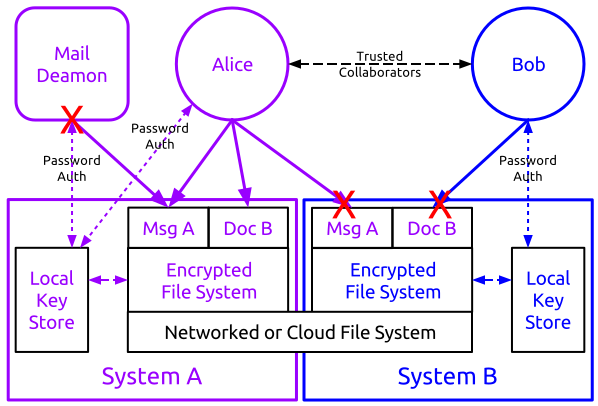
\includegraphics[width=.5\textwidth]
                        {./figs/pdf/App-FS-Traditional-Layered.pdf}
        \caption{Traditional Layered File System Encryption}
        \label{fig:FS-traditional-layered}
      \end{center}
    \end{subfigure}
    \begin{subfigure}{\textwidth}
      \begin{center}
        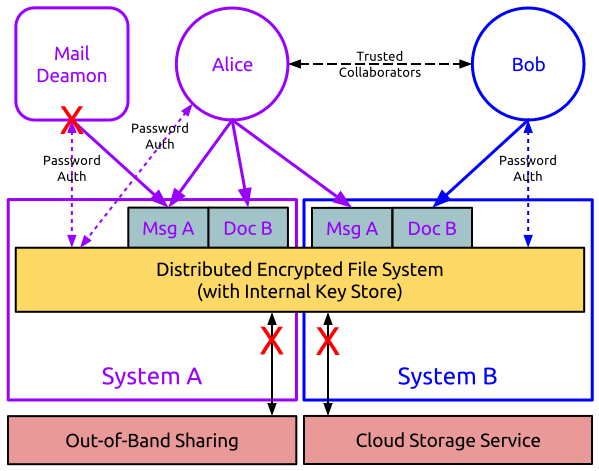
\includegraphics[width=.5\textwidth]
                        {./figs/pdf/App-FS-Traditional-Integrated.pdf}
        \caption{Traditional Integrated File System Encryption}
        \label{fig:FS-traditional-integrated}
      \end{center}
    \end{subfigure}
  \end{center}
  \caption{Traditional File System Encryption Challenges}
  \label{fig:FS-traditional}
\end{figure}

Unfortunately, existing encrypted file systems fail to provide
encryption in a flexible manner appropriately matched to the ways in
which users expect to utilize them. Layered encryption solutions like
dm-crypt~\cite{dm-crypt} and eCryptfs~\cite{eCryptfs, Halcrow} suffer
from a number of limitations related to their tightly-coupled local
key storage and access management components. As Figure
\ref{fig:FS-traditional-layered} shows, these systems work fine for an
individual user like Alice wishing to secure items like her mail or
documents and access them from a single machine. But they quickly
break down when trying to move beyond the simple single-user,
single-device use case. Alice can not access her encrypted mail file
across a networked file system from System B since System B has no
access to the encryption keys stored on System A. Furthermore, she can
not share a work document with a trusted collaborator like Bob, since
Bob neither has access to her encryption keys stored on System A nor
the password required to unlock these keys. A non-interactive process
like the Mail Daemon is also unable to leverage these encrypted file
systems due to the inability of such services to securely and
interactively provide a password to unlock the keys needed to decrypt
local files.

While full stack distributed encrypted file systems such as
OceanStore~\cite{Kubiatowicz2000}, Plutus~\cite{Kallahalla2003},
Cumulus4j~\cite{cumulus4j}, or Tahoe~\cite{Wilcox-O'Hearn2008} tend to
succeed in solving some of the sharing and distribution problems
inherent in local secure file systems, they still lack the flexibility
required to address the full range of desired use cases. Figure
\ref{fig:FS-traditional-integrated} shows some of the remaining issues
inherent in distributed solutions. Notably, while multi-user use cases
are better supported, non-interactive use cases are still a
challenge. Furthermore, full stack distributed file systems tend to be
wedded with specific storage systems and thus lack support for
Cloud-based ``Storage as a Service'' offerings or alternate underlying
storage technologies. These systems also lack support for most forms
of ``out-of-band'' file sharing (via e-mail, USB flash drives, etc)
due to the inability of actors outside of the integrated stack to
access the necessary encryption keys.

\begin{figure}[!tb]
  \vspace{5ex}
  \begin{center}
    \begin{subfigure}{\textwidth}
      \begin{center}
        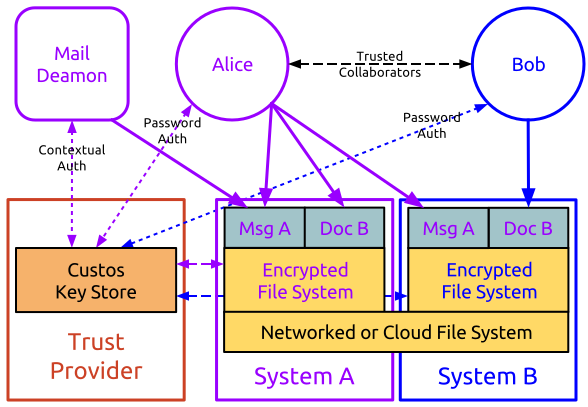
\includegraphics[width=.5\textwidth]
                        {./figs/pdf/App-FS-Custos-Layered.pdf}
        \caption{Layered File System Encryption with Custos}
        \label{fig:FS-custos-layered}
      \end{center}
    \end{subfigure}
    \begin{subfigure}{\textwidth}
      \begin{center}
        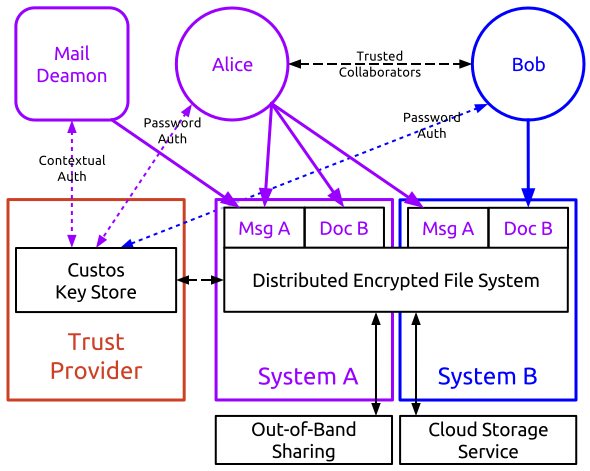
\includegraphics[width=.5\textwidth]
                        {./figs/pdf/App-FS-Custos-Integrated.pdf}
        \caption{Integrated File System Encryption with Custos}
        \label{fig:FS-custos-integrated}
      \end{center}
    \end{subfigure}
  \end{center}
  \caption{File System Encryption with Custos}
  \label{fig:FS-custos}
\end{figure}

Custos aims to improve upon existing encrypted file systems by
separating key storage and access control from data storage and
encryption. Instead of storing keys themselves, a Custos-backed file
system will hand off all key storage duties to a Custos server,
leaving the file system to focus on data encryption and storage while
Custos focuses on access control. In doing so, Custos can support a
variety of extensible authentication mechanisms enabling a range of
access control rules. Its flexible, centralized nature also strives to
simplify multi-device syncing and multi-user sharing, as well as
provide support for a variety of modern and future use cases.

Figure \ref{fig:FS-custos-layered} shows how traditional layered file
systems (Figure \ref{fig:FS-traditional-layered}) might be improved
through incorporation with Custos. The logically centralized nature of
Custos allows Alice to now access her files on a range of devices. It
also allows her to grant access to Bob, her trusted
collaborator. Custos's support for flexible authentication schemes
including context-based authentication allows it to even support
non-interactive key access by systems like a mail daemon. In all
cases, Custos provides a single point for controlling, revoking, and
auditing access.

Figure \ref{fig:FS-custos-integrated} shows how traditional integrated
file systems (Figure \ref{fig:FS-traditional-integrated}) might be
improved through the incorporation of Custos. Custos's centralization
and flexible authentication mechanisms allow for simple multi-user,
multi-device, and non-interactive access. In addition, mechanisms like
out-of-band sharing are now possible, since encrypted files may be
moved around or stored on cloud services without having to worry about
ensuring future access to their corresponding encryption keys. These
keys are all stored in Custos, and will be potentially available
wherever the file needs to be accessed.

\begin{table}[!tb]
  \vspace{5ex}
  \begin{center}
    \tabulinesep = 5pt
    \begin{tabu} to \textwidth
      { | X[1.5,c,m]
        | X[1,c,m]
        | X[1,c,m]
        | X[1,c,m]
        | X[1,c,m]
        | }
      \hline
      & \textbf{Unencrypted File System}
      & \textbf{Local Encrypted File System}
      & \textbf{Distributed Encrypted File System}
      & \textbf{Custos Encrypted File System}
      \\ \hline
      \textbf{Encrypt Files}
      & No & Yes & Yes & Yes
      \\ \hline
      \textbf{Local Access Control}
      & No & Yes & Maybe & No
      \\ \hline
      \textbf{Remote Access Control}
      & No & No & Maybe & Yes
      \\ \hline
      \textbf{Local Access Auditing}
      & No & Maybe & Maybe & No
      \\ \hline
      \textbf{Remote Access Auditing}
      & No & No & Maybe & Yes
      \\ \hline
      \textbf{Flexible Authentication}
      & N/A & No & No & Yes
      \\ \hline
      \textbf{Share Files (In-Band)}
      & N/A & No & Yes & Yes
      \\ \hline
      \textbf{Share Files (Out-of-Band)}
      & Yes & No & No & Yes
      \\ \hline
      \textbf{Multi-Device Access}
      & Yes & No & No & Yes
      \\ \hline
      \textbf{Trusted 3rd Party}
      & No & No & Maybe & Maybe
      \\ \hline
      \end{tabu}
  \end{center}
  \caption{Feature Comparison of Encrypted File System Architectures}
  \label{tab:comp-fs}
\end{table}

Table \ref{tab:comp-fs} shows a side-by-side comparison of the
features of various encrypted file system architectures. In general,
Custos is able to leverage its flexibility and centralized nature to
enable use cases not possible in traditional file systems. I will
discuss the manner in which Custos achieves these features in Chapter
\ref{chap:platform}.

\subsection{Data Centers}

Modern data centers are a lesson in ephemeral state. The
commoditization of ``cloud'' computing means that pretty much anyone
can create a virtual server, use it for a bit, and then destroy it
again to avoid paying for more than they need. The Cloud's ``pay only
for what you need'' business case manifests as a highly dynamic,
impermanent ecosystem where resources are in constant churn. This has
created a slew of management systems~\cite{chef, salt, puppet}
designed to handle the need for persistent configuration and
management across a range of ephemeral resources.

\begin{figure}[!tb]
  \vspace{5ex}
  \begin{center}
    \begin{subfigure}{\textwidth}
      \begin{center}
        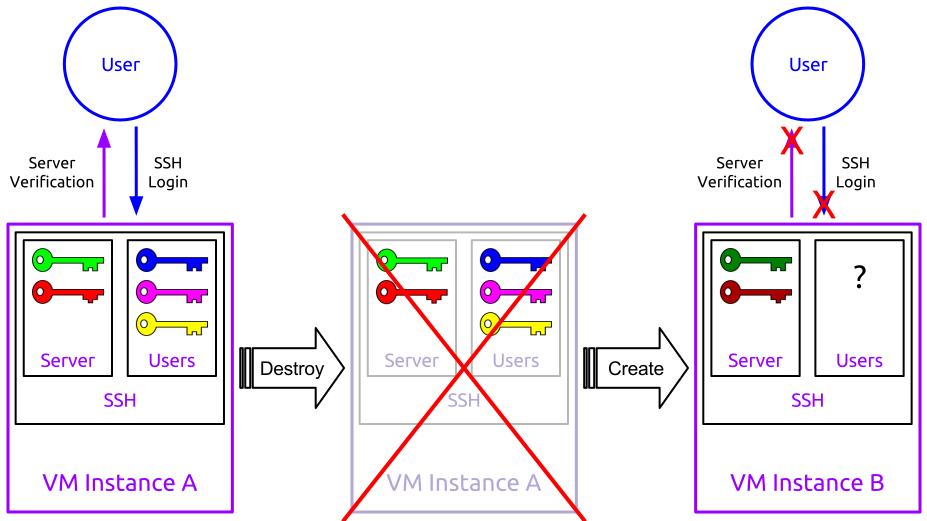
\includegraphics[width=.5\textwidth]
                        {./figs/pdf/App-DC-Traditional.pdf}
        \caption{Challenges Managing Keys in Traditional Data Centers}
        \label{fig:DC-traditional}
      \end{center}
    \end{subfigure}
    \begin{subfigure}{\textwidth}
      \begin{center}
        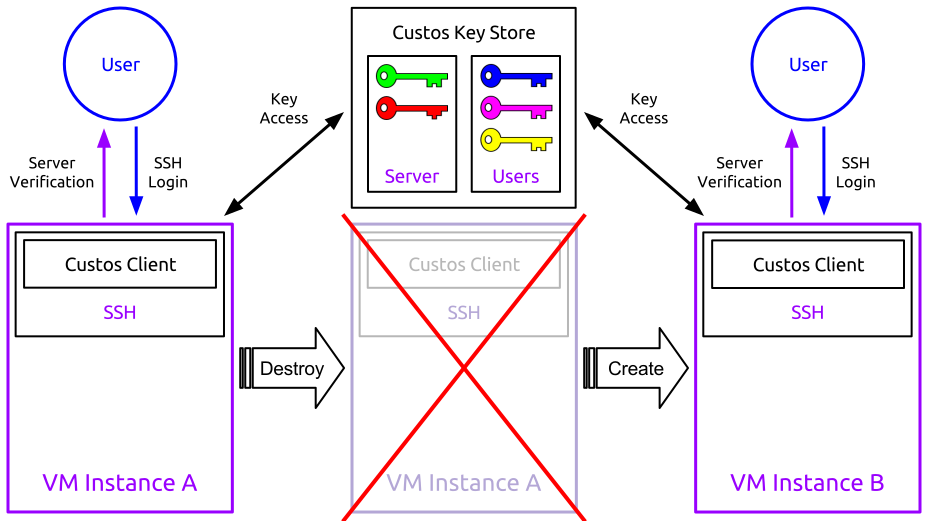
\includegraphics[width=.5\textwidth]
                        {./figs/pdf/App-DC-Custos.pdf}
        \caption{Offloading Key Management to Custos Resolves Issues}
        \label{fig:DC-custos}
      \end{center}
    \end{subfigure}
  \end{center}
  \caption{Data Center Application Key Management}
  \label{fig:DC}
\end{figure}

What is currently missing, however, is a secure method for storing
sensitive configuration data and distributing it to the appropriate
resource. Often virtual machines and other cloud resources will
require a variety of cryptographic keys (e.g. SSH, SSL, AES, VPN, etc)
to perform their desired roles. Today, these keys must either be
regenerated on each VM, stored in a non-secure traditional
configuration service, or manually copied to each machine from a
secure location. What we need is a secure Secret Storage as a Service
platform through which ephemeral cloud resources can easily gain
access to the sensitive keys they require. Custos can be used as the
basis of such a service.

Take, for example, SSH. As Figure \ref{fig:DC-traditional} shows, SSH
can pose a challenge in the data center where new instances of VMs are
constantly being created and destroyed. Since VMs tend to generate
their SSH keys at install time\footnote{generating SSH keys at install
  time poses other challenges related to the size of the entropy
  pool~\cite{Heninger2012} that switching to Custos-stored persistent
  SSH keys could also help combat.}, each VM instance will present a
separate SSH server key, making it difficult for the user to verify
the identity of the VM when trying to connect. Furthermore,
administrators who use SSH user keys in place of login passwords must
manually reload each VM with the necessary user keys in order to grant
users access. This issue can become quite the burden, especially when
dealing with a multitude of VMs. Custos could be used to provide a
centralized store for SSH keys across VM instances as shown in Figure
\ref{fig:DC-custos}, providing users immediate and simple access to
new VM resources as soon as they are created. It would also allow VMs
to maintain their cryptographic identities across instances, helping
users vet a machine before logging in, and would provide
administrators with a centralized system for managing SSH access to
all of their VMs.

In addition to SSH key storage, Custos can serve a wide range of
additional data center use cases. For instance, Custos could be used
as described in the file system section (above) to enable use of
encrypted file systems between multiple VMs or across VM
instances. Custos could be used to enable access to secure VPN
systems, proving users with access to various cloud resources by
storing the necessary cryptographic keys these resources
require. Likewise, Custos could be used to store and coordinate access
to private SSL keys across a domain of web services. In all of these
cases, Custos's flexible authentication capabilities, centralized
nature, and auditing capabilities would contribute to easing the use
of cryptographic services in the data center.

\begin{table}[!tb]
  \vspace{5ex}
  \begin{center}
    \tabulinesep = 5pt
    \begin{tabu} to \textwidth
      { | X[1.5,c,m]
        | X[1,c,m]
        | X[1,c,m]
        | X[1,c,m]
        | }
      \hline
      & \textbf{DC without Key Storage Service}
      & \textbf{DC with Generic Key Storage Service}
      & \textbf{DC with Custos Key Storage Service}
      \\ \hline
      \textbf{Provide SSH Access to New Resources}
      & No & Maybe & Yes
      \\ \hline
      \textbf{Provide VPN Access to New Resources}
      & No & Maybe & Yes
      \\ \hline
      \textbf{Provide SSL Access to New Resources}
      & No & Maybe & Yes
      \\ \hline
      \textbf{Enable Use of Shared Encrypted Volumes}
      & No & Maybe & Yes
      \\ \hline
      \textbf{Enable Use of Persistent Encrypted Volumes}
      & No & Yes & Yes
      \\ \hline
      \textbf{Centralized Access Auditing}
      & No & Yes & Yes
      \\ \hline
      \textbf{Flexible Authentication}
      & N/A & Maybe & Yes
      \\ \hline
      \textbf{API-Based Key Access}
      & N/A & Maybe & Yes
      \\ \hline
      \textbf{Trusted 3rd Party}
      & N/A & Maybe & Maybe
      \\ \hline
      \end{tabu}
  \end{center}
  \caption{Feature Comparison of Data Center Key Management Architectures}
  \label{tab:comp-dc}
\end{table}

Table \ref{tab:comp-dc} shows a comparison of data center capabilities
across various key storage systems. Custos has the potential to
greatly simply many cloud operations by allowing applications and
systems to offload key management to a dedicated key management
service. Custos's flexible authentication and access control make it
compatible with a wide range of potential cloud applications. Custos's
auditing capabilities can help cloud providers meet various compliance
standards and ensure that users feel comfortable storing their data
securely in the cloud.

\subsection{End-User Secret Stores}

Another possible application for Custos is as a cloud-based end-user
secret manager. In reality, Custos is always a form of secret
store. But in encryption-related applications, the secretes Custos is
storing are private encryption keys, not any actual user data
directly. Forgoing the encryption-related applications for a moment,
Custos's secret store capabilities can be leveraged directly to store
generic end-user data. While Custos has been designed to optimize the
storage of encryption keys, it is perfectly capable of storing other
secrets as well. In such a situation, Custos could be used to store
passwords, personal data, or any other secrets.

In this arrangement Custos could be used to replace existing Password
mangers like LastPass~\cite{lastpass}, 1Password~\cite{onepassword},
or iCloud's Keychain~\cite{icloud}. Instead of mapping encrypted data
IDs to encryption keys as has been discussed thus far, Custos could be
used to map URLs of web services requesting password to the password
itself. A Custos client could then be used to retrieve the password
for a given site when necessary. Such a solution could leverage
Custos's existing flexible authentication scheme and central key:value
store to securely keep track of user passwords.

A similar arrangement could be used to protect personal user data
(i.e. SSN, DoB, name, email, phone, address, etc). Many websites
request this data on a regular basis for everything from simple
account creation to online commerce to secondary authentication
(e.g. when you forget and reset your password). Today, users must
manually enter this data when required, causing both a data entry
burden and making it difficult to keep data in sync and up to date
across disparate sites. Custos could solve these problems by creating
a central repository of personal data. Instead of reentering this data
on multiple sites, users could simply leverage the Custos access
control semantics to grant access to specific pieces of data to
specific sites. In addition to avoiding the need to constantly reenter
this data, this system would also make it easy for users to keep data
up to date, allowing them to do things like update their mailing
address in a single location, allowing all sites to which they have
granted address access to simply read the new address from Custos when
required. Such a system might even discourage services from storing
copies of user data directly at all, as it would be easier to stay
up-to-date with user data changes if the service simply queried Custos
for the most up to date version of the data each time it is
required. Users could monitor website access to data via Custos,
allowing them to stay apprised of how their data was being used.

It is worth noting, however, that unlike the encryption key storage
applications, using Custos directly as a secret store reduces Custos
to a single-point-of-failure trust model. In most encryption key
storage scenarios, an adversary would need to have access to both the
encrypted data and the corresponding encryption keys stored on Custos
to actually access a user's information. In the direct secret store
case, this multi-party attack is no longer necessary. Instead, any
adversary who gains access to Custos will have direct access to any
secrets stored there. Thus it might be desirable to keep Custos as a
specialized encryption key store and defer to separate systems for
storing actual secrets, which could then be encrypted with keys from
Custos. We might even consider using two separate Custos providers to
accomplish such a system: one provider would securely store a set of
encrypted user secrets (passwords, user info, etc) while the other
provider would store the encryption keys corresponding to these
secrets. This would maintain a multi-party trust model, making it more
difficult for a single bad actor to compromise user data. It would
also allow one service to optimize the storage of actual encrypted
secretes (which may not necessarily require the level of access
control Custos provides) while Custos optimizes the storage of
encryption keys as in prior applications.

\begin{table}[!tb]
  \vspace{5ex}
  \begin{center}
    \tabulinesep = 5pt
    \begin{tabu} to \textwidth
      { | X[1.5,c,m]
        | X[1,c,m]
        | X[1,c,m]
        | X[1,c,m]
        | X[1,c,m]
        | }
      \hline
      & \textbf{Per-Service Secret Store}
      & \textbf{Traditional Cloud Secret Store}
      & \textbf{Custos Direct Secret Store}
      & \textbf{Custos Backed Secret Store}
      \\ \hline
      \textbf{Share Data Across Services}
      & No & Maybe & Yes & Yes
      \\ \hline
      \textbf{Update Data Across Services}
      & No & Maybe & Yes & Yes
      \\ \hline
      \textbf{Centralized Access Control}
      & No & Maybe & Yes & Yes
      \\ \hline
      \textbf{Centralized Access Auditing}
      & No & Maybe & Yes & Yes
      \\ \hline
      \textbf{Flexible Authentication}
      & N/A & No & Yes & Yes
      \\ \hline
      \textbf{API-Based Secret Access}
      & N/A & No & Yes & Maybe
      \\ \hline
      \textbf{Single-Point of Trust}
      & Yes & Yes & Yes & No
      \\ \hline
      \textbf{Trusted 3rd Party}
      & Yes & Maybe & Maybe & Maybe
      \\ \hline
      \end{tabu}
  \end{center}
  \caption{Feature Comparison of Secret Store Architectures}
  \label{tab:comp-ss}
\end{table}

Table \ref{tab:comp-ss} shows a side-by-side comparison of the
features of various secret store architectures. As you can see, Custos
has many of the benefits of a traditional cloud secret store (password
manager, etc), with the additional benefits of a standardized API and
flexible authentication. Custos could be leveraged, either directly or
as the encryption key store, to greatly simplify end-user secret
storage, reducing user effort while increasing user security.

\section{Threat Model}

Like any system, the Custos architecture operates with certain
assumptions as the basis of its security profile. These assumptions
form the Custos security model: what must be trusted, what kind of
attacks Custos can defend against, etc.

\subsection{Model}

At the core of the Custos security model is the assumption that a
Custos providers are themselves trusted and secure. Custos does not
inherently strive to protect users from malevolent Custos providers
who might intentionally or accidentally leak data stored in Custos,
fail to enforce the requested ACLs, or make other violations of the
intended Custos design. Custos provides a means for separating trust
from functionality and isolating trust to dedicated providers, but
Custos does not eliminate the need for trust all together. It only
aims to provide more control over where the trust in placed. This is
the price we pay for the ease-of-use benefits Custos provides. A
trusted Custos provider is assumed to:

\begin{packed_item}
\item Securely store Custos secrets (key:value pairs)
\item Faithfully enforce all Custos access control requirements
\item Securely implement proper verification of authentication attributes
\item Properly implement appropriate secure communication protocols where
  required (SSL, etc)
\item Accurately log all Custos access information and make this data
  available to the user.
\item Ensure that servers running Custos are kept physically and
  digitally secure to resist attacks on both Custos and non-Custos
  components
\end{packed_item}

Beyond the security of the Custos provider and the data stored there,
the threat model for a given Custos-backed application is largely a
function of the applications' implementation. For example, a
Custos-integrated file system may opt to maintain a local cache of
encryption keys to allow offline file access. Such behavior, however,
would open an additional attack vector whereby an adversary must only
compromise a local key cache to gain file access without ever having
to compromise a Custos server itself. Custos, however, is designed to
be flexible, which means leaving such trade-offs up to each individual
application.

Like most encrypted file systems, encryption key-access via Custos is
a one-time play: once a user or system has been granted access to a
key, it must be assumed that the user or system will always have
access to the data associated with that key since they can decrypt,
copy, and store the such data indefinitely. There is no reliable way
to revoke access to a key or the data it protects once access is
granted once.

Custos also leaves authentication requirements and access control up
to each user. Thus, the burden of ensuring that data is being
adequately protected, either directly in Custos or via encryption with
the necessary keys stored in Custos, lies with the user configuring
the necessary authentication and access control requirements. Custos
aims to make it easy for the user to create and maintain access
control requirements for specific data, but Custos can not guarantee
that the user is making intelligent decisions related to the
protection of their data. Custos provides flexibility and ease of use,
which should maximize protection while minimizing usage errors, but
some level of user intelligence and responsibility is still required
for secure Custos use.

\subsection{Mitigation}

The Custos threat model does have its limitations. That said, there
are various ways to mitigate these restrictions and further increase
the security of a Custos-backed system.

While Custos does require Custos providers to generally be trusted, it
is possible to manage this trust. As was mentioned previously,
building an open market of competing Custos providers would tie
trustworthiness to monetary competition. If a user finds that a
specific Custos provider is prone to misbehavior, she can take her
secrets elsewhere. If a user reports misbehaving providers to other
market consumers, she can damage the reputation of such providers and
in the process, discourage other users from using said providers. The
market for secret storage will create an incentive not to misbehave,
and the user can rely on this incentive as the basis of provider
trust.

If a user is unwilling to place full trust in a single Custos provider
at all, she has a few options. First, when Custos is used to store
encrypted data keys and not the data itself, a Custos provider only
ever has access to part of the required information to actually access
the user's data. While the Custos provider may hold the encryption
keys, unless they can also gain access to the underlying data itself,
these keys are useless. Thus, by storing her data locally or with a
separate provider than the Custos provider, a Custos user can help
reduce the damage a misbehaving Custos provider could cause.

\begin{figure}[!tb]
  \vspace{5ex}
  \begin{center}
    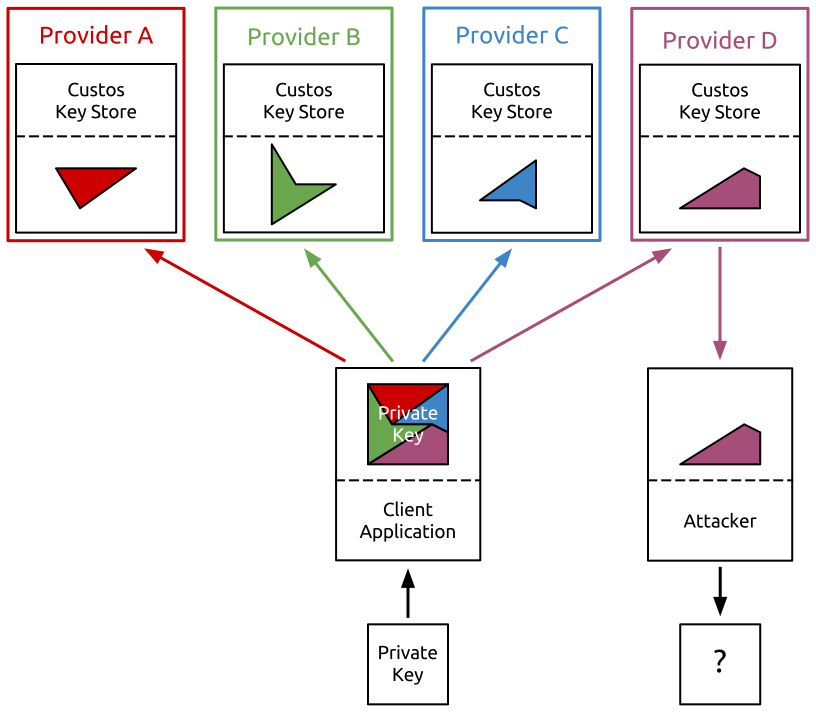
\includegraphics[width=.75\textwidth]
                    {./figs/pdf/Arch-Sharded.pdf}
  \end{center}
  \caption{Sharding Trust Across Multiple Providers}
  \label{fig:arch-sharded}
\end{figure}

Second, a user can opt to securely shard her Custos data (encryption
keys, etc) across multiple, non-cooperating Custos providers as shown
in Figure \ref{fig:arch-sharded}. A variety of secure secret-sharing
systems have been proposed~\cite{Shamir1979, Resch2011, Krawczyk1993},
and these system could be leveraged by Custos-backed applications to
split Custos data between multiple Custos providers. Such a system
does not require the Custos's providers to even be aware that they are
only storing a part of a larger secret. Instead, Custos providers
behave as they always would, but the user must query multiple Custos
providers to reassemble the full secret. Such a strategy also
mitigates a Custos provider being offline or unavailable, since many
secret sharing system support reassembly using only K of a larger set
of N keys. I believe many Custos application will leverage secret
sharing to avoid placing trust in a single Custos provider or relying
on a single Custos provider's availability.

A Custos user could also opt to self-host her own Custos server. This
might be an appropriate approach for situations requiring retaining
local control over all data for regulatory or compliance related
reasons. While this does not relieve the user from the burden of
properly securing her own Custos server, it does eliminate the need to
trust a third party. For many users, operating their own Custos server
might be too complex a burden. These users will instead opt to consume
Custos services from one or more trust providers. But for user's
capable and interested in self-hosting a Custos install, there is no
reason they can not opt to take that route.

It's also possible for clients to locally encrypt Custos-stored data
before shipping it off to a Custos provider. This action, however
would negate many of the benefits Custos provides and reintroduce the
inflexible-use-case problems inherent in existing encryption systems
due to the chicken-and-the-egg problem that would come along with
it. If you encrypt encryption keys stored on Custos, where do you
store the encryption keys' encryption keys? Like the secret sharing
option, Custos providers do not need to be aware of whether or not the
data they hold has already been encrypted on the client side. For some
applications, client-side encryption of Custos data may be
appropriate, but I don't feel it will be the most common case due to
the additional flexibility and key storage problems it poses.

The traditional revocation problems associated with using encryption
(e.g. inability to revoke access to data a user has already decrypted)
are not unique to Custos. As such, Custos can mitigate this issue in
the same manner most system do: through versioning, rotation, and lazy
revocation~\cite{Kallahalla2003}. While Custos can not revoke access
to data that has already been decrypted and read, Custos can revoke
access to all future versions or modifications of that data. This is
accomplished by having a Custos application re-encrypt the data with a
new key each time it is updated. These new keys are then uploaded to
Custos leveraging Custos's versioning support. When a user revokes
access to a Custos object, Custos blocks all future access to any
versions of that object uploaded after the revocation occurred. Custos
can't force users to un-see data they have seen, but it can help
prevent users from seeing changes to that data. In a similar manner to
versioning, Custos's auditing capabilities also make it possible for
users to revoke access to data that has never been previously
accessed, and to asses the effect revoking access will have on the
basis of who has and who has not previously access the data.

In terms of Custos server security, Custos's backing data store could
be built atop existing Hardware Security Module (HSM)
platforms~\cite{fips140}. Such systems utilize hardware-based
constraints to control access to the data they store. They can help
mitigate the damage that a compromised Custos server would pose by
limiting access to the underlying Custos data stored on such a
server. Several cloud platforms are already beginning to offer access
to cloud-based HSM resources that might be appropriate for Custos
server implementations~\cite{amazon-hsm}. Whether or not a Custos
server is backed by such technology could be one of the determining
factors users use to evaluate whether to use a specific Custos
provider and thus could drive the market price such a provider might
be able to charge.

%%  LocalWords:  dm Plutus LastPass iCloud's VM's
